\documentclass[10pt,a4paper]{amsart}
\usepackage{amsmath,amssymb,amsthm,graphicx}
\usepackage{amsmath,amssymb,graphicx,xcolor,mathtools}
\title{Tietze transformations preserve presented sets and are complete under choice}
\author{Samuel Mimram, Émile Oleon}
\date{doi:10.4230/LIPIcs.FSCD.2025.30; CC BY4.0 (official paper and diagrams)}
\begin{document}
\maketitle
\noindent\textit{Editorial note.} Source https://drops.dagstuhl.de/entities/document/10.4230/LIPIcs.FSCD.2025.30. © Samuel Mimram and Émile Oleon, CC BY4.0. Complete author natural-language proof and original diagrams retained.\par\medskip
\noindent\textit{Editorial note.} The completeness direction retains the original axiom of choice and the author disclosure that §2.3 has not yet been fully formalized in Agda; collection does not add a formalization.\par\medskip
\noindent\textit{Allowed standard prerequisites (editorial).}\begin{itemize}
\item Homotopy type theory with univalence, higher inductive coequalizers and propositional/set truncation. Full author §1 and exactsource references retained.
\item Axiom of choice for the completeness direction, in the exact formulation of author Axiom18. Author §2.3 explicitly states this assumption and that the section is not yet fully formalized in Agda.
\end{itemize}\medskip
% BEGIN S1
 
\par\medskip\noindent\textbf{1 1-polygraphs}\par
 
% BEGIN S1.p1
 
Before introducing 1-polygraphs, we first need to present the (quite trivial) 0-dimensional variant. A 0-polygraph $P$ is simply a type whose elements are called $0$-generators. A sphere $(x,y)$ in a 0-polygraph $P$ is a pair of elements of $P$, and we write $\operatorname{S}P$ for the type of such objects. If we write $\operatorname{S}^{0}=\{0,1\}$ for the type with two elements, corresponding to the canonical 0-sphere, it can be noted that a sphere in a 0-polygraph $P$ corresponds to an arrow $\operatorname{S}^{0}\to P$. Given a $0$-polygraph $P$, we call $\|P\|_{-1}$ the proposition presented by $P$.\par
 
% END S1.p1
 
% BEGIN S1.SS1
 
\par\medskip\noindent\textbf{1.1 Internal and external 1-polygraphs}\par
 
% BEGIN S1.SS1.SSS0.P0.SPx1
 
\par\medskip\noindent\textbf{1-polygraphs.}\par
 
% BEGIN S1.SS1.SSS0.P0.SPx1.p1
 
A 1-polygraph $P$ consists of a 0-polygraph $\operatorname{U}P$ (the underlying 0-polygraph of $P$) together with a function $\operatorname{S}{\operatorname{U}P}\to\mathcal{U}$, which to any sphere $(x,y)$ in the underlying 0-polygraph associates a type $P(x,y)$ whose elements are called the 1-generators of the 1-polygraph. In other words, 1-polygraphs correspond to type-theoretic directed graphs. A 1-polygraph is discrete when all the types $\operatorname{U}P$ and $P(x,y)$ are sets. In the following, a sphere in $\operatorname{U}P$ is called a 0-sphere of $P$.\par
 
% END S1.SS1.SSS0.P0.SPx1.p1
 
% END S1.SS1.SSS0.P0.SPx1
 
% BEGIN S1.SS1.SSS0.P0.SPx2
 
\par\medskip\noindent\textbf{1-generators.}\par
 
% BEGIN S1.SS1.SSS0.P0.SPx2.p1
 
The elements of $\operatorname{U}P$ are called 0-generators or 0-cells of $P$. We sometimes write $\operatorname{S}_{0}P:=\operatorname{S}\operatorname{U}P$ for the 0-spheres, as well as $P_{0}:=\operatorname{U}P$ and $P_{1}:=\Sigma((x,y):\operatorname{S}_{0}P).P(x,y)$ for the type of 0- and 1-generators of $P$. We also write $\partial^{-},\partial^{+}:P_{1}\to P_{0}$ for the source and target functions (defined by $\partial^{-}:=\pi\circ\pi$ and $\partial^{+}:=\pi^{\prime}\circ\pi$).\par
 
% END S1.SS1.SSS0.P0.SPx2.p1
 
% END S1.SS1.SSS0.P0.SPx2
 
% BEGIN S1.SS1.SSS0.P0.SPx3
 
\par\medskip\noindent\textbf{1-cells.}\par
 
% BEGIN S1.SS1.SSS0.P0.SPx3.p1
 
Given a 1-polygraph $P$ and a $0$-sphere $(x,y)$, we write $P^{*}(x,y)$ for the type of 1-cells in $P$ from $x$ to $y$. This family of types is defined inductively as the smallest one such that\par
  
\par\noindent  $\blacksquare$ 
% BEGIN S1.I1.i1.p1
 
for every 0-cell $x:\operatorname{U}P$, we have a 1-cell $\operatorname{id}_{x}:P^{*}(x,x)$,\par
 
% END S1.I1.i1.p1
 
 
\par\noindent  $\blacksquare$ 
% BEGIN S1.I1.i2.p1
 
for every 0-cells $x,y,z:\operatorname{U}P$, 1-generator $a:P(x,y)$ and $1$-cell $u:P^{*}(y,z)$, we have a 1-cell $a::u:P^{*}(x,z)$,\par
 
% END S1.I1.i2.p1
 
 
\par\noindent  $\blacksquare$ 
% BEGIN S1.I1.i3.p1
 
for every 0-cells $x,y,z:\operatorname{U}P$, 1-generator $a:P(y,x)$ and $1$-cell $u:P^{*}(y,z)$, we have a 1-cell $a::^{\prime}u:P^{*}(x,z)$.\par
 
% END S1.I1.i3.p1
 
  
Informally, cells in $P^{*}(x,y)$ are undirected paths from $x$ to $y$ in the graph corresponding to $P$ (where the two last cases respectively correspond to taking an arrow $a$ forward and backward). In the following, we often write $a:x\to y$ for a 1-generator $a:P(x,y)$ and $u:x\overset{*}{\to}y$ for a 1-cell $u:P^{*}(x,y)$.\par
 
% END S1.SS1.SSS0.P0.SPx3.p1
 
% END S1.SS1.SSS0.P0.SPx3
 
% BEGIN S1.SS1.SSS0.P0.SPx4
 
\par\medskip\noindent\textbf{Composition.}\par
 
% BEGIN S1.SS1.SSS0.P0.SPx4.p1
 
Given two 1-cells $u:x\overset{*}{\to}y$ and $v:y\overset{*}{\to}z$, we define their composite $u\cdot{}v:x\overset{*}{\to}z$ by induction on $u$ by\par
    $\displaystyle\operatorname{id}\cdot{}v$ $\displaystyle:=v$ $\displaystyle(a::u)\cdot{}v$ $\displaystyle:=a::(u\cdot{}v)$ $\displaystyle(a::^{\prime}u)\cdot{}v$ $\displaystyle:=a::^{\prime}(u\cdot{}v)$    
% END S1.SS1.SSS0.P0.SPx4.p1
 
% BEGIN Thmtheorem1
 
\par\medskip\noindent\textbf{Lemma 1 ([13, comp0-assoc]).}\par
 
% BEGIN Thmtheorem1.p1
 
Composition is associative and unital.\par
 
% END Thmtheorem1.p1
 
% END Thmtheorem1
 
% BEGIN S1.SS1.SSS0.P0.SPx4.p2
 
Given a 1-cell $u:x\overset{*}{\to}y$, we define its opposite $u^{\mathrm{op}}:y\overset{*}{\to}x$ by induction on $u$ by\par
    $\displaystyle\operatorname{id}^{\mathrm{op}}$ $\displaystyle:=\operatorname{id}$ $\displaystyle(a::u)^{\mathrm{op}}$ $\displaystyle:=a\mathbin{\overline{::}^{\prime}}u^{\mathrm{op}}$ $\displaystyle(a::^{\prime}u)^{\mathrm{op}}$ $\displaystyle:=a\mathbin{\overline{::}}u^{\mathrm{op}}$    
where $a\mathbin{\overline{::}}u$, which corresponds to appending $a$ to $u$, is defined by\par
    $\displaystyle a\mathbin{\overline{::}}\operatorname{id}$ $\displaystyle:=a::\operatorname{id}$ $\displaystyle a\mathbin{\overline{::}}(b::u)$ $\displaystyle:=b::(a\mathbin{\overline{::}}u)$ $\displaystyle a\mathbin{\overline{::}}(b::^{\prime}u)$ $\displaystyle:=b::^{\prime}(a\mathbin{\overline{::}}u)$    
and $a\mathbin{\overline{::}^{\prime}}u$, corresponding to appending $a$ backward to $u$, is defined similarly.\par
 
% END S1.SS1.SSS0.P0.SPx4.p2
 
% END S1.SS1.SSS0.P0.SPx4
 
% BEGIN S1.SS1.SSS0.P0.SPx5
 
\par\medskip\noindent\textbf{Spheres.}\par
 
% BEGIN S1.SS1.SSS0.P0.SPx5.p1
 
A sphere $s$ in a 1-polygraph $P$ consists of a $0$-sphere $(x,y)$ together with a pair of 1-cells $f,g:x\overset{*}{\to}y$. The underlying 0-sphere $(x,y)$ is noted $\operatorname{U}s$. The cell $f$ (resp. $g$) is called the source (resp. target) of $s$ and noted $\partial^{-}s$ (resp. $\partial^{+}s$), so that the sphere $s$ is the triple $(\operatorname{U}s,\partial^{-}s,\partial^{+}s)$. We write $\operatorname{S}P$ for type of spheres in a $1$-polygraph.\par
 
% END S1.SS1.SSS0.P0.SPx5.p1
 
% END S1.SS1.SSS0.P0.SPx5
 
% BEGIN S1.SS1.SSS0.P0.SPx6
 
\par\medskip\noindent\textbf{Coherent 1-cells.}\par
 
% BEGIN S1.SS1.SSS0.P0.SPx6.p1
 
In the definition of 1-cell, we think of $a::-$ and $a::^{\prime}-$ as respectively precomposing by the 1-cell $a$ and its inverse. However, nothing enforces that they are actually inverse operations, i.e. that we have\par
    $\displaystyle a::^{\prime}a::u$ $\displaystyle=u$ $\displaystyle a::a::^{\prime}u$ $\displaystyle=u$    
for any 1-generator $a$ and 1-cell $u$ of suitable types. We define the types of coherent 1-cells $P^{\sim}(x,y)$, indexed by 0-spheres $(x,y)$, as the quotient of the types of 1-cells $P^{*}(x,y)$ under the congruence generated by the above relations. This type is the “right” definition for the 1-cells of $P$, in the sense that it gives a description of the free groupoid generated by $P$ [9]. However, non coherent 1-cells provides representatives for those which are often simpler to work with. Namely, by definition of coherent 1-cells as a quotient of 1-cells, we have\par
 
% END S1.SS1.SSS0.P0.SPx6.p1
 
% BEGIN Thmtheorem2
 
\par\medskip\noindent\textbf{Lemma 2.}\par
 
% BEGIN Thmtheorem2.p1
 
For $x,y:\operatorname{U}P$, the canonical map $f:P^{*}(x,y)\to P^{\sim}(x,y)$ is a surjection, i.e. the type $\|\operatorname{hfib}_{f}(u)\|_{-1}$ is inhabited for any $u:P^{\sim}(x,y)$.\par
 
% END Thmtheorem2.p1
 
% END Thmtheorem2
 
% END S1.SS1.SSS0.P0.SPx6
 
% END S1.SS1
 
% BEGIN S1.SS2
 
\par\medskip\noindent\textbf{1.2 Geometric realization}\par
 
% BEGIN S1.SS2.p1
 
We introduce the “geometric realization” of a 1-polygraph $P$, which can be thought of as a type-theoretical graph with $P_{0}$ as vertices and $P_{1}$ as edges. The set presented by $P$ is then defined as the type of connected components of this graph.\par
 
% END S1.SS2.p1
 
% BEGIN S1.SS2.SSS0.P0.SPx1
 
\par\medskip\noindent\textbf{Geometric realization.}\par
 
% BEGIN S1.SS2.SSS0.P0.SPx1.p1
 
Given a 1-polygraph $P$ its geometric realization $\overline{P}$ is the higher inductive type generated by the two constructors\par
    $\displaystyle\iota:\operatorname{U}P$ $\displaystyle\to\overline{P}$ $\displaystyle\gamma:((x,y):\operatorname{S}_{0}P)\to P(x,y)$ $\displaystyle\to\iota x=\iota y$    
More abstractly, it corresponds to the pushout on the left or to the coequalizer on the right\par
    
\begin{center}
\includegraphics[width=0.95\linewidth,height=0.42\textheight,keepaspectratio]{graph-01.pdf}\end{center}
    
where the horizontal arrow $f$ sends an edge $a:x\to y$ and $0$ (resp. $1$) to $x$ (resp. $y$), which corresponds to attaching 1-cells to a 0-dimensional cell complex. The associated induction principle is the following.\par
 
% END S1.SS2.SSS0.P0.SPx1.p1
 
% BEGIN Thmtheorem3
 
\par\medskip\noindent\textbf{Proposition 3.}\par
 
% BEGIN Thmtheorem3.p1
 
Suppose given an arbitrary type $A$. Any two functions $f_{0}:P_{0}\to A$ and $f_{1}:(((x,y),a):P_{1})\to f_{0}(x)=f_{0}(y)$ induce a unique function $f:\overline{P}\to A$ such that $f\circ\iota=f_{0}$ and $f\circ\gamma=f_{1}$. We also have the expected dependent generalization.\par
 
% END Thmtheorem3.p1
 
% END Thmtheorem3
 
% BEGIN S1.SS2.SSS0.P0.SPx1.p2
 
By partial evaluation, the map $\gamma$ induces, for $(x,y):\operatorname{S}_{0}P$, a map $\gamma_{x,y}:P(x,y)\to\iota x=\iota y$, which extends as a map on cells $\gamma^{*}_{x,y}:P^{*}(x,y)\to\iota x=\iota y$ defined by induction by\par
    $\displaystyle\gamma^{*}_{x,x}(\operatorname{id})$ $\displaystyle:=\operatorname{refl}$ $\displaystyle\gamma^{*}_{z,y}(a::u)$ $\displaystyle:=\gamma a\cdot{\gamma^{*}_{x,y}(u)}$ $\displaystyle\gamma^{*}_{z,y}(a::^{\prime}u)$ $\displaystyle:=\gamma a^{-}\cdot{\gamma^{*}_{x,y}(u)}$    
Moreover, since this definition is compatible with the relations for coherent 1-cells, for every sphere $(x,y):\operatorname{S}_{0}P$ we have the following.\par
 
% END S1.SS2.SSS0.P0.SPx1.p2
 
% BEGIN Thmtheorem4
 
\par\medskip\noindent\textbf{Lemma 4.}\par
 
% BEGIN Thmtheorem4.p1
 
The map $\gamma^{*}_{x,y}$ induces a map $\gamma^{\sim}_{x,y}:P^{\sim}(x,y)\to\iota x=\iota y$.\par
 
% END Thmtheorem4.p1
 
% END Thmtheorem4
 
% BEGIN S1.SS2.SSS0.P0.SPx1.p3
 
This map is an equivalence, so it provides a characterization of the paths in geometric realizations of graphs [13, KvR/1Polygraph/PathPresentation.agda]:\par
 
% END S1.SS2.SSS0.P0.SPx1.p3
 
% BEGIN Thmtheorem5
 
\par\medskip\noindent\textbf{Theorem 5.}\par
 
% BEGIN Thmtheorem5.p1
 
The map $\gamma^{\sim}_{x,y}:P^{\sim}(x,y)\to\iota x=\iota y$ is an equivalence.\par
 
% END Thmtheorem5.p1
 
% END Thmtheorem5
 
% END S1.SS2.SSS0.P0.SPx1
 
% BEGIN S1.SS2.SSS0.P0.SPx2
 
\par\medskip\noindent\textbf{Proof.}\par
 
% BEGIN S1.SS2.SSS0.P0.SPx2.p1
 
A map $\iota x=\iota y\to P^{\sim}(x,y)$ can be defined using the elimination principle for paths in $\overline{P}$ given in [9, Theorem 3], and both can be shown to be mutually inverse by induction. $\hfill\blacktriangleleft$\par
 
% END S1.SS2.SSS0.P0.SPx2.p1
 
% END S1.SS2.SSS0.P0.SPx2
 
% BEGIN S1.SS2.SSS0.P0.SPx3
 
\par\medskip\noindent\textbf{Presented set.}\par
 
% BEGIN S1.SS2.SSS0.P0.SPx3.p1
 
The set presented by a 1-polygraph $P$ is the set of connected components of its geometric realization $\|\overline{P}\|_{0}$. This notion is to be understood as an analogue of a group presentation with generators and relations, but shifted down by one dimension: here, the 0-cells of $P$ are the generators of the presented set, and the 1-cells are the relations.\par
 
% END S1.SS2.SSS0.P0.SPx3.p1
 
% BEGIN Thmtheorem6
 
\par\medskip\noindent\textbf{Example 6.}\par
 
% BEGIN Thmtheorem6.p1
 
Consider the polygraph $P$ with $\operatorname{U}P=\mathbb{Z}$ and one relation $a_{n}:n\to n+2$ for $n\in\mathbb{Z}$. The presented set is $\mathbb{Z}_{2}$.\par
 
% END Thmtheorem6.p1
 
% END Thmtheorem6
 
% BEGIN S1.SS2.SSS0.P0.SPx3.p2
 
We now prove some technical lemmas that will be useful later on.\par
 
% END S1.SS2.SSS0.P0.SPx3.p2
 
% BEGIN Thmtheorem7
 
\par\medskip\noindent\textbf{Lemma 7.}\par
 
% BEGIN Thmtheorem7.p1
 
For $x,y:\operatorname{U}P$ and $p:|\iota(x)|_{0}=|\iota(y)|_{0}$ in $\|\overline{P}\|_{0}$, there merely exists a 1-cell $x\overset{*}{\to}y$ in $P$.\par
 
% END Thmtheorem7.p1
 
% END Thmtheorem7
 
% END S1.SS2.SSS0.P0.SPx3
 
% BEGIN S1.SS2.SSS0.P0.SPx4
 
\par\medskip\noindent\textbf{Proof.}\par
 
% BEGIN S1.SS2.SSS0.P0.SPx4.p1
 
By [19, Theorem 7.3.12], the type $|\iota(x)|_{0}=|\iota(y)|_{0}$ coincides with $\|\iota(x)=\iota(y)\|_{-1}$. Since we are eliminating to a proposition, we can suppose given a path $p:\iota(x)=\iota(y)$ which by Theorem 5 induces a coherent cell $\tilde{p}:P^{\sim}(x,y)$, and we conclude by Lemma 2. $\hfill\blacktriangleleft$ The following shows that we can pick a representative 0-cell in every connected component [13, has-repr]:\par
 
% END S1.SS2.SSS0.P0.SPx4.p1
 
% BEGIN Thmtheorem8
 
\par\medskip\noindent\textbf{Proposition 8.}\par
 
% BEGIN Thmtheorem8.p1
 
The type $\Pi(x:\|\overline{P}\|_{0}).\|\Sigma(\hat{x}:\operatorname{U}P).|\iota(\hat{x})|_{0}=x\|_{-1}$ is inhabited.\par
 
% END Thmtheorem8.p1
 
% END Thmtheorem8
 
% END S1.SS2.SSS0.P0.SPx4
 
% BEGIN S1.SS2.SSS0.P0.SPx5
 
\par\medskip\noindent\textbf{Proof.}\par
 
% BEGIN S1.SS2.SSS0.P0.SPx5.p1
 
Any proposition being a set [19, Lemma 3.3.4], it is enough to construct a map $f:\Pi(x:\overline{P}).\|\Sigma(\hat{x}:\operatorname{U}P).\iota(\hat{x})=x\|_{-1}$ which can be done by using the elimination principle of $\overline{P}$ (Proposition 3). Namely, we define, for $x:\operatorname{U}P$, $f(\iota(x)):=|(x,\operatorname{refl}_{\iota(x)})|_{-1}$ and, for $x,y:\operatorname{U}P$ and $a:P(x,y)$, the path associated to it by $f$ is canonically defined by the fact that we are eliminating to a proposition. $\hfill\blacktriangleleft$\par
 
% END S1.SS2.SSS0.P0.SPx5.p1
 
% END S1.SS2.SSS0.P0.SPx5
 
% END S1.SS2
 
% END S1


% BEGIN S2
 
\par\medskip\noindent\textbf{2 Tietze transformations}\par
 
% BEGIN S2.p1
 
Tietze transformations originate from the work of Tietze [18] who defined two transformations on group presentations:\par
  (T0)  
% BEGIN S2.I1.ix1.p1
 
adding a definable generator,\par
 
% END S2.I1.ix1.p1
  (T1)  
% BEGIN S2.I1.ix2.p1
 
adding a derivable relation.\par
 
% END S2.I1.ix2.p1
   
The equivalence relation they induce, the Tietze equivalence, characterizes when two presentations give rise to the same group, up to isomorphism. These transformations have then been generalized to a variety of contexts, including the very general one of polygraphs [1, 5] for presentations of (higher) categories, and have as well been shown to provide a interesting notion of weak equivalence [7]. Their fundamental property can be decomposed in two parts:\par
  
\par\noindent  $\blacksquare$ 
% BEGIN S2.I2.i1.p1
 
correctness: any two presentations which are Tietze equivalent present the same structure,\par
 
% END S2.I2.i1.p1
 
 
\par\noindent  $\blacksquare$ 
% BEGIN S2.I2.i2.p1
 
completeness: any two presentations of the same structure are Tietze equivalent.\par
 
% END S2.I2.i2.p1
 
  
Here, we think of a 1-polygraph $P$ as presenting the set $\|\overline{P}\|_{0}$, and we define elementary transformations as explained above. We then show that they are correct and complete with respect to the presented set.\par
 
% END S2.p1
 
% BEGIN S2.SS1
 
\par\medskip\noindent\textbf{2.1 Definition}\par
 
% BEGIN S2.SS1.p1
 
We define the two following families of Tietze transformations, which transform a given 1-polygraph $P$ into another 1-polygraph, by attaching cells to it:\par
  (T0)  
% BEGIN S2.I3.ix1.p1
 
Add a definable 0-generator: given a type $X$ and a function $\partial:X\to\operatorname{U}P$, we construct the polygraph $P{\uparrow_{0}}\partial$ defined, for $(x,y):\operatorname{S}_{0}P$, by\par
    $\displaystyle\operatorname{U}(P{\uparrow_{0}}\partial)$ $\displaystyle:=\operatorname{U}P\sqcup X$ $\displaystyle(P{\uparrow_{0}}\partial)(x,y)$ $\displaystyle:=\begin{cases}P(x,y)&\text{if $x:\operatorname{U}P$ and $y:\operatorname{U}P$}\\
x=\partial(y)&\text{if $x:\operatorname{U}P$ and $y:X$}\\
\bot&\text{otherwise}\end{cases}$    
% END S2.I3.ix1.p1
  (T1)  
% BEGIN S2.I3.ix2.p1
 
Add a derivable relation: given a function $\partial:\operatorname{S}_{0}P\to\mathcal{U}$ and a family of functions $\partial_{x,y}:\partial(x,y)\to(x\overset{*}{\to}y)$ indexed by 0-spheres $(x,y):\operatorname{S}_{0}P$, we construct the polygraph $P{\uparrow_{1}}\partial$ defined, for $(x,y):\operatorname{S}_{0}P$, by\par
    $\displaystyle\operatorname{U}(P{\uparrow_{1}}\partial)$ $\displaystyle:=\operatorname{U}P$ $\displaystyle(P{\uparrow_{1}}\partial)(x,y)$ $\displaystyle:=P(x,y)\sqcup\partial(x,y)$    
% END S2.I3.ix2.p1
   
A transformation (T0) consists in adding, for every element $x:X$, a new 0-generator $x$ to the polygraph together with a 1-generator $\tau_{x}:\partial x\to x$:\par
    
\begin{center}
\includegraphics[width=0.95\linewidth,height=0.42\textheight,keepaspectratio]{graph-02.pdf}\end{center}
    
with $y\overset{\text{def}}{=}\partial x$, and $\tau_{x}$ is a notation for the element $\operatorname{refl}_{x}:(P{\uparrow_{0}}\partial)(y,x)$. A transformation (T1) consists in adding, for every $x,y:X$ and $a:\partial(x,y)$, a 1-generator $a:x\to y$:\par
    
\begin{center}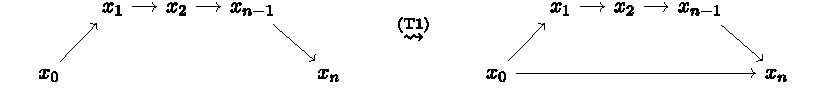
\includegraphics[width=0.95\linewidth,height=0.42\textheight,keepaspectratio]{graph-03.pdf}\end{center}
    
It can be observed that we have a new hole after performing a transformation (T1), which justifies the importance of the set-truncation in the definition of the presented set. Note that the functions $\partial_{x,y}$ are not used in order to define $Q$ in (T1), but they will be necessary to show the correctness of the transformation below. For instance, if we did not require those, we could make any polygraph coherent by taking $\partial(x,y)=\top$ for any $(x,y):\operatorname{S}_{0}P$.\par
 
% END S2.SS1.p1
 
% BEGIN Thmtheorem9
 
\par\medskip\noindent\textbf{$\blacktriangleright$ Remark 9.}\par
 
% BEGIN Thmtheorem9.p1
 
We could also consider a weaker notion of transformation (T1) where we only require the existence of the 1-cell associated to an added 1-generator, i.e. type the function as $\partial_{x,y}:\partial(x,y)\to\|x\overset{*}{\to}y\|_{-1}$. This variant would in fact be enough for the subsequent developments here.\par
 
% END Thmtheorem9.p1
 
% END Thmtheorem9
 
% BEGIN Thmtheorem10
 
\par\medskip\noindent\textbf{Example 10.}\par
 
% BEGIN Thmtheorem10.p1
 
We have the following series of Tietze transformations:\par
    
\begin{center}
\includegraphics[width=0.95\linewidth,height=0.42\textheight,keepaspectratio]{graph-04.pdf}\end{center}
    
% END Thmtheorem10.p1
 
% END Thmtheorem10
 
% BEGIN S2.SS1.p2
 
Under the Grothendieck duality between type families and fibrations [19, Section 4.8], the Tietze transformations (T1) can reformulated as follows (a similar reformulation for (T0) could also be given):\par
 
% END S2.SS1.p2
 
% BEGIN Thmtheorem11
 
\par\medskip\noindent\textbf{Proposition 11.}\par
 
% BEGIN Thmtheorem11.p1
 
Transformations (T1) are equivalent to the following:\par
  (T1’)  
% BEGIN S2.I4.ix1.p1
 
Given a type $X:\mathcal{U}$ and function $\partial:X\to\Sigma((x,y):\operatorname{S}_{0}P).P^{*}(x,y)$, we construct the polygraph $P{\uparrow_{1}}\partial$ with $\operatorname{U}(P{\uparrow_{1}}\partial):=\operatorname{U}P$ and, for $(x,y):\operatorname{S}P$,\par
    \[(P{\uparrow_{1}}\partial)(x,y):=P(x,y)\sqcup\operatorname{hfib}_{\pi\circ\partial}(x,y)\]    
% END S2.I4.ix1.p1
   
% END Thmtheorem11.p1
 
% END Thmtheorem11
 
% BEGIN S2.SS1.p3
 
We define the Tietze equivalence as the equivalence relation generated by (T0) and (T1).\par
 
% END S2.SS1.p3
 
% BEGIN S2.SS1.SSS0.P0.SPx1
 
\par\medskip\noindent\textbf{Transformations for 0-polygraphs.}\par
 
% BEGIN S2.SS1.SSS0.P0.SPx1.p1
 
The notion of Tietze transformation generalizes to polygraphs in any dimension. In particular, for 0-polygraphs, it can be formulated as follows. An elementary Tietze transformation of 0-polygraphs consists in\par
  (T0)  
% BEGIN S2.I5.ix1.p1
 
Given a 0-polygraph $P$, a type $X$ and a function $\partial:X\to P$, we consider the 0-polygraph $P{\uparrow_{0}}\partial:=P\sqcup X$.\par
 
% END S2.I5.ix1.p1
   
Two 0-polygraphs are Tietze equivalent when they are related by the smallest equivalence relation identifying $P$ with $P{\uparrow_{0}}\partial$ for any $P$ and $\partial$.\par
 
% END S2.SS1.SSS0.P0.SPx1.p1
 
% BEGIN Thmtheorem12
 
\par\medskip\noindent\textbf{Proposition 12.}\par
 
% BEGIN Thmtheorem12.p1
 
There exists a Tietze equivalence between two 0-polygraphs $P$ and $Q$ if and only if they present the same proposition, i.e. $\|P\|_{-1}=\|Q\|_{-1}$.\par
 
% END Thmtheorem12.p1
 
% END Thmtheorem12
 
% END S2.SS1.SSS0.P0.SPx1
 
% END S2.SS1
 
% BEGIN S2.SS2
 
\par\medskip\noindent\textbf{2.2 Correctness}\par
 
% BEGIN S2.SS2.p1
 
Our aim is now to show the correctness property for Tietze transformations of 1-polygraphs: equivalent 1-polygraphs present the same set.\par
 
% END S2.SS2.p1

% BEGIN Thmtheorem13
 
\par\medskip\noindent\textbf{Theorem 13 (Correctness).}\par
 
% BEGIN Thmtheorem13.p1
 
Given two Tietze equivalent 1-polygraphs $P$ and $Q$, we have $\|\overline{P}\|_{0}=\|\overline{Q}\|_{0}$.\par
 
% END Thmtheorem13.p1
 
% END Thmtheorem13

% BEGIN S2.SS2.p2
 
By induction on the equivalence, it is enough to show the result when $Q$ is obtained form $P$ by a Tietze transformation (T0) or (T1), which we do below. Throughout the section, we suppose fixed a 1-polygraph $P$. We first show that transformations (T0) are correct [13, tietze0-correct]:\par
 
% END S2.SS2.p2
 
% BEGIN Thmtheorem14
 
\par\medskip\noindent\textbf{Proposition 14.}\par
 
% BEGIN Thmtheorem14.p1
 
Given a type $X$ and a function $\partial:X\to\operatorname{U}P$, we have $\|\overline{P}\|_{0}=\|\overline{P{\uparrow_{0}}\partial}\|_{0}$.\par
 
% END Thmtheorem14.p1
 
% END Thmtheorem14
 
% BEGIN S2.SS2.SSS0.P0.SPx1
 
\par\medskip\noindent\textbf{Proof.}\par
 
% BEGIN S2.SS2.SSS0.P0.SPx1.p1
 
By definition of $P{\uparrow_{0}}\partial$ and its geometric realization, we have a coequalizer\par
    
\begin{center}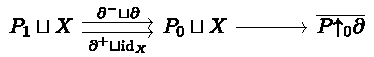
\includegraphics[width=0.95\linewidth,height=0.42\textheight,keepaspectratio]{graph-05.pdf}\end{center}
    
By computing the coequalizer partially on the left component of the coproduct, we find that $\overline{P{\uparrow_{0}}\partial}$ is the coequalizer of $\begin{matrix}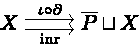
\includegraphics[width=0.24\linewidth,height=0.12\textheight,keepaspectratio]{graph-06.pdf}\end{matrix}$. From which we easily deduce $\overline{P{\uparrow_{0}}\partial}=\overline{P}$. $\hfill\blacktriangleleft$ The transformations (T0) actually preserve, not only the presented set, but also the geometric realization. We now show that transformations (T1) are correct [13, tietze1-correct]:\par
 
% END S2.SS2.SSS0.P0.SPx1.p1
 
% BEGIN Thmtheorem15
 
\par\medskip\noindent\textbf{Proposition 15.}\par
 
% BEGIN Thmtheorem15.p1
 
Given a type $X$, a function $\partial:\operatorname{S}_{0}P\to\mathcal{U}$, and a family of functions $\partial_{x,y}:\partial(x,y)\to(x\overset{*}{\to}y)$ indexed by 0-spheres $(x,y):\operatorname{S}_{0}P$, we have $\|\overline{P}\|_{0}=\|\overline{P{\uparrow_{1}}\partial}\|_{0}$.\par
 
% END Thmtheorem15.p1
 
% END Thmtheorem15
 
% END S2.SS2.SSS0.P0.SPx1
 
% BEGIN S2.SS2.SSS0.P0.SPx2
 
\par\medskip\noindent\textbf{Proof.}\par
 
% BEGIN S2.SS2.SSS0.P0.SPx2.p1
 
By using the induction principle of geometric realization (Proposition 3), we can define a map $s:\overline{P}\to\overline{P{\uparrow_{1}}\partial}$ by\par
    $\displaystyle s(\iota(x))$ $\displaystyle:=\iota(x)$ $\displaystyle\operatorname{ap}_{s}(\gamma(a))$ $\displaystyle:=\gamma(\mathrm{inl}(a))$    
for $x:P_{0}$ and $a:x\to y$ in $P_{1}$. Conversely, we define a map $r:\overline{P{\uparrow_{1}}\partial}\to\overline{P}$ by induction by\par
    $\displaystyle r(\iota(x))$ $\displaystyle:=\iota(x)$ $\displaystyle\operatorname{ap}_{r}(\gamma(\mathrm{inl}(a)))$ $\displaystyle:=\gamma(a)$ $\displaystyle\operatorname{ap}_{r}(\gamma(\mathrm{inr}(b)))$ $\displaystyle:=\gamma^{*}_{x,y}(\partial_{x,y}(b))$    
for $x:P_{0}$, $a:x\to y$ in $P_{1}$, and $b:\partial(x,y)$ for some $(x,y):\operatorname{S}_{0}P$. By induction, they can be shown to form a section-retraction pair, which induces an equivalence on the 0-truncations. $\hfill\blacktriangleleft$\par
 
% END S2.SS2.SSS0.P0.SPx2.p1
 
% END S2.SS2.SSS0.P0.SPx2

% BEGIN S2.SS3
 
\par\medskip\noindent\textbf{2.3 Completeness}\par
 
% BEGIN S2.SS3.p1
 
We now show a converse completeness result: any two 1-polygraphs presenting the same set are Tietze equivalent. Throughout the section, we thus suppose fixed two 1-polygraphs $P$ and $Q$ such that we have an equality $\|\overline{P}\|_{0}=\|\overline{Q}\|_{0}$. We write $f:\|\overline{P}\|_{0}\to\|\overline{Q}\|_{0}$ and $g:\|\overline{Q}\|_{0}\to\|\overline{P}\|_{0}$ for the components of the induced equivalence between the two types. Our goal is to show that the 1-polygraphs $P$ and $Q$ are equivalent. We should point out that this part has not (yet) been fully formalized in Agda.\par
 
% END S2.SS3.p1
 
% BEGIN S2.SS3.p2
 
In this section, we also need to suppose that the axiom of choice is satisfied. It is known to be consistent with homotopy type theory [19, Lemma 3.8.2], and can be formulated as follows:\par
 
% END S2.SS3.p2
 
% BEGIN Thmtheorem18
 
\par\medskip\noindent\textbf{Axiom 18.}\par
 
% BEGIN Thmtheorem18.p1
 
The axiom of choice assumes an inhabitant of the type\par
    \[\Pi(x:A).\|B(x)\|_{-1}\to\|\Pi(x:A).B(x)\|_{-1}\]    
for every $A:\mathcal{U}$ and $B:A\to\mathcal{U}$.\par
 
% END Thmtheorem18.p1
 
% END Thmtheorem18
 
% BEGIN S2.SS3.p3
 
Informally, this axiom states that any family of merely inhabited types is itself merely inhabited.\par
 
% END S2.SS3.p3
 
% BEGIN S2.SS3.p4
 
Proving the completeness result in Theorem 22 below requires us to first show some technical lemmas. We begin by observing that the maps $f$ and $g$ can be lifted to maps between the underlying types of 0-generators.\par
 
% END S2.SS3.p4
 
% BEGIN Thmtheorem19
 
\par\medskip\noindent\textbf{Proposition 19.}\par
 
% BEGIN Thmtheorem19.p1
 
There merely exist maps $\hat{f}:\operatorname{U}P\to\operatorname{U}Q$ and $\hat{g}:\operatorname{U}Q\to\operatorname{U}P$ such that\par
    $\displaystyle|\iota(\hat{f}(x))|_{0}$ $\displaystyle=f(|\iota(x)|_{0})$ $\displaystyle|\iota(\hat{g}(y))|_{0}$ $\displaystyle=g(|\iota(y)|_{0})$    
for $x:\operatorname{U}P$ and $y:\operatorname{U}Q$.\par
 
% END Thmtheorem19.p1
 
% END Thmtheorem19
 
% BEGIN S2.SS3.SSS0.P0.SPx1
 
\par\medskip\noindent\textbf{Proof.}\par
 
% BEGIN S2.SS3.SSS0.P0.SPx1.p1
 
We define a map $f^{\prime}$ by\par
    
\begin{center}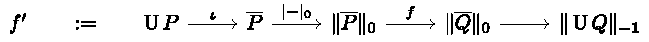
\includegraphics[width=0.95\linewidth,height=0.42\textheight,keepaspectratio]{graph-09.pdf}\end{center}
    
where the rightmost map is the one defined in Proposition 8. By the axiom of choice, we deduce the existence of a map\par
    \[\hat{f}:\|\operatorname{U}P\to\operatorname{U}Q\|_{-1}\]    
satisfying the required identity. The map $\hat{g}$ is constructed similarly. $\hfill\blacktriangleleft$ We then show that any 1-generator in $P$ induces a 1-cell in $Q$ between the image of its endpoints.\par
 
% END S2.SS3.SSS0.P0.SPx1.p1
 
% BEGIN Thmtheorem20
 
\par\medskip\noindent\textbf{Lemma 20.}\par
 
% BEGIN Thmtheorem20.p1
 
Given a 1-generator $a:x\to y$ in $P$, there merely exists a 1-cell $\hat{f}(x)\overset{*}{\to}\hat{f}(y)$ in $Q$, that we call $\hat{f}(a)$ in the following.\par
 
% END Thmtheorem20.p1
 
% END Thmtheorem20
 
% END S2.SS3.SSS0.P0.SPx1
 
% BEGIN S2.SS3.SSS0.P0.SPx2
 
\par\medskip\noindent\textbf{Proof.}\par
 
% BEGIN S2.SS3.SSS0.P0.SPx2.p1
 
By definition of the geometric realization, the 1-generator $a$ induces an equality $\gamma(a):\iota(x)=\iota(y)$ in $\overline{P}$, and thus, by functoriality of $f$ and $|\cdot|_{0}$, an equality\par
    \[\operatorname{ap}_{f}(|\gamma(a)|_{0}):f(|\iota(x)|_{0})=f(|\iota(y)|_{0})\]    
Since, by Proposition 19, we have $|\iota(\hat{f}(x))|_{0}=f(|\iota(x)|_{0})$ (and similarly for $y$), there is an equality\par
    \[|\iota(\hat{f}(x))|_{0}=|\iota(\hat{f}(y))|_{0}\]    
and we deduce, by Lemma 7, the existence of a 1-cell $\hat{f}(x)\overset{*}{\to}\hat{f}(y)$ as desired. $\hfill\blacktriangleleft$ Furthermore, the maps $\hat{f}$ and $\hat{g}$ are mutually inverse modulo post-composition by $|\iota(\cdot)|_{0}$.\par
 
% END S2.SS3.SSS0.P0.SPx2.p1
 
% BEGIN Thmtheorem21
 
\par\medskip\noindent\textbf{Lemma 21.}\par
 
% BEGIN Thmtheorem21.p1
 
For every $x:\operatorname{U}P$, we have $|\iota(\hat{g}(\hat{f}(x)))|_{0}=|\iota(x)|_{0}$ in $\|\overline{P}\|_{0}$ (and similarly, we have $|\iota(\hat{f}(\hat{g}(x)))|_{0}=|\iota(y)|_{0}$ for $y:\operatorname{U}Q$).\par
 
% END Thmtheorem21.p1
 
% END Thmtheorem21
 
% END S2.SS3.SSS0.P0.SPx2
 
% BEGIN S2.SS3.SSS0.P0.SPx3
 
\par\medskip\noindent\textbf{Proof.}\par
 
% BEGIN S2.SS3.SSS0.P0.SPx3.p1
 
Given $x:\operatorname{U}P$, by Proposition 19 and the fact that $f$ and $g$ are mutually inverse maps, we have $|\iota(\hat{g}(\hat{f}(x)))|_{0}=g(|\iota(\hat{f}(x))|_{0})=g(f(|\iota(x)|_{0}))=|\iota(x)|_{0}$. $\hfill\blacktriangleleft$ Finally, we can show the completeness theorem.\par
 
% END S2.SS3.SSS0.P0.SPx3.p1

% BEGIN Thmtheorem22
 
\par\medskip\noindent\textbf{Theorem 22 (Completeness).}\par
 
% BEGIN Thmtheorem22.p1
 
Consider two 1-polygraphs $P$ and $Q$ such that $\|\overline{P}\|_{0}=\|\overline{Q}\|_{0}$. Then, assuming the axiom of choice, $P$ and $Q$ are merely Tietze-equivalent.\par
 
% END Thmtheorem22.p1
 
% END Thmtheorem22

% END S2.SS3.SSS0.P0.SPx3
 
% BEGIN S2.SS3.SSS0.P0.SPx4
 
\par\medskip\noindent\textbf{Proof.}\par
 
% BEGIN S2.SS3.SSS0.P0.SPx4.p1
 
Starting from the polygraph $P$, we are going to construct step-by-step a polygraph $P^{3}$ that contains both $P$ and $Q$ and is Tietze-equivalent to $P$ (and thus to $Q$ by symmetry).\par
  
\par\noindent  1. 
% BEGIN S2.I6.i1.p1
 
We add the 0-generators of $Q$. We write $P^{1}:=P{\uparrow_{0}}\hat{g}$ for the polygraph obtained from $P$ by performing a transformation (T0) with $\hat{g}:\operatorname{U}Q\to\operatorname{U}P$. Its type of 0-generators is $\operatorname{U}P\sqcup\operatorname{U}Q$ and the 1-generators are those of $P$ together with one 1-generator $\hat{g}(x)\to x$ for every $x:\operatorname{U}Q$.\par
 
% END S2.I6.i1.p1
 
 
\par\noindent  2. 
% BEGIN S2.I6.i2.p1
 
We add the relations from $P$ to $Q$. Given a 0-generator $x:\operatorname{U}P$, we claim that there exists a 1-cell $\hat{f}(x)\overset{*}{\to}x$ in $P^{1}$. By previous step, we have a cell\par
    \[a:\hat{g}(\hat{f}(x))\to\hat{f}(x)\]    
Moreover, by Lemma 21, we have $|\iota(\hat{g}(\hat{f}(x)))|_{0}=|\iota(x)|_{0}$, so the type $\|\hat{g}(\hat{f}(x))\overset{*}{\to}x\|_{-1}$ is inhabited by Lemma 7, and we can suppose that we actually have a 1-cell\par
    \[u:\hat{g}(\hat{f}(x))\overset{*}{\to}x\]    
because we are eliminating to a proposition. Hence, we can define a 1-cell $w_{x}:\hat{f}(x)\overset{*}{\to}x$ by $w_{x}:=a::^{\prime}u$ for every $x:\operatorname{U}P$. Finally, we consider the function\par
    $\displaystyle\partial:\operatorname{U}P^{1}$ $\displaystyle\to\Sigma((x,y):\operatorname{S}_{0}P^{1}).(x\overset{*}{\to}y)$     $\displaystyle x$ $\displaystyle\mapsto((\hat{f}(x),x),w_{x})$    
and define $P^{2}:=P^{1}{\uparrow_{1}}\partial$ by a transformation (T1’), see Proposition 11.\par
 
% END S2.I6.i2.p1
 
 
\par\noindent  3. 
% BEGIN S2.I6.i3.p1
 
We add the 1-generators of $Q$. Given a 1-generator $b:x\to y$ in $Q$, we have 1-generators $a:g(x)\to x$ and $c:g(y)\to y$ in $P^{2}$ (by the first step), and we have the 1-cell $g(a):g(x)\overset{*}{\to}g(y)$ by Lemma 20. We therefore have a 1-cell\par
    \[a\cdot{}g(b)\cdot{}c:x\overset{*}{\to}y\]    
in $Q$. This induces a function\par
    \[\partial:\Sigma((x,y):\operatorname{S}_{0}Q).Q(x,y)\to\Sigma((x,y):\operatorname{S}_{0}P^{2}).(x\overset{*}{\to}y)\]    
which, to $(x,y):\operatorname{S}_{0}Q$ and $a:Q(x,y)$ associates the pair consisting of $(x,y)$ (or rather its image under the canonical inclusion) and the 1-cell constructed above. Finally, we define $P^{3}:=P^{2}{\uparrow_{1}}\partial$ by a transformation (T1’).\par
 
% END S2.I6.i3.p1
 
  
In the 1-polygraph $P^{3}$ constructed above, the 0-generators are $\operatorname{U}P^{3}=\operatorname{U}P\sqcup\operatorname{U}Q$ and the 1-generators are (up to canonical inclusion): those of $P$, those of $Q$ (by the third step), $\hat{g}(x)\to x$ for $x:\operatorname{U}Q$ (by the first step), $\hat{f}(x)\to x$ for $x:\operatorname{U}P$ (by the second step). By exchanging the roles of $P$ and $Q$, we see that $Q$ is also Tietze-equivalent to the above 1-polygraph (up to standard isomorphisms such as commutation of coproducts). By transitivity, we conclude that $P$ and $Q$ are Tietze-equivalent. $\hfill\blacktriangleleft$\par
 
% END S2.SS3.SSS0.P0.SPx4.p1
 
% END S2.SS3.SSS0.P0.SPx4
 
% END S2.SS3

\begin{thebibliography}{99}

% BEGIN bib
 
\par\medskip\noindent\textbf{References}\par
  
\par\noindent  [1]  Dimitri Ara, Albert Burroni, Yves Guiraud, Philippe Malbos, François Métayer, and Samuel Mimram.  Polygraphs: from rewriting to higher categories.  Cambridge University Press, 2025.  
 
\par\noindent  [2]  Franz Baader and Tobias Nipkow.  Term rewriting and all that.  Cambridge University Press, 1998.  
 
\par\noindent  [3]  Christopher J Dean, Eric Finster, Ioannis Markakis, David Reutter, and Jamie Vicary.  Computads for weak $\omega$-categories as an inductive type.  Advances in Mathematics, 450, 2024.  
 
\par\noindent  [4]  Yves Guiraud and Philippe Malbos.  Identities among relations for higher-dimensional rewriting systems.  In Operads 2009, volume 26 of Séminaires et congrès, pages 145–161. Société Mathématique de France, 2013.  
 
\par\noindent  [5]  Yves Guiraud and Philippe Malbos.  Polygraphs of finite derivation type.  Mathematical Structures in Computer Science, 28(2):155–201, 2018.  doi:10.1017/S0960129516000220.  
 
\par\noindent  [6]  Allen Hatcher.  Algebraic Topology.  Cambridge University Press, 2002.  
 
\par\noindent  [7]  Simon Henry and Samuel Mimram.  Tietze equivalences as weak equivalences.  Applied Categorical Structures, 30(3):453–483, 2022.  doi:10.1007/S10485-021-09662-W.  
 
\par\noindent  [8]  Donald E. Knuth and Peter B. Bendix.  Simple word problems in universal algebras.  In Computational problems in abstract algebra, pages 263–297. Pergamon, 1970.  
 
\par\noindent  [9]  Nicolai Kraus and Jakob von Raumer.  Path spaces of higher inductive types in homotopy type theory.  In 2019 34th Annual ACM/IEEE Symposium on Logic in Computer Science (LICS), pages 1–13. IEEE, 2019.  doi:10.1109/LICS.2019.8785661.  
 
\par\noindent  [10]  Nicolai Kraus and Jakob von Raumer.  A rewriting coherence theorem with applications in homotopy type theory.  Mathematical Structures in Computer Science, 32(7):982–1014, 2022.  doi:10.1017/S0960129523000026.  
 
\par\noindent  [11]  Yves Lafont.  A new finiteness condition for monoids presented by complete rewriting systems (after Craig C. Squier).  Journal of Pure and Applied Algebra, 98(3):229–244, 1995.  
 
\par\noindent  [12]  Yves Lafont, François Métayer, and Krzysztof Worytkiewicz.  A folk model structure on omega-cat.  Advances in Mathematics, 224(3):1183–1231, 2010.  
 
\par\noindent  [13]  Samuel Mimram.  Polygraphs in Agda.  Software, swhId: swh:1:dir:27f2a0c3a496b72c3f4cd458ab51ea174f448eb7 (visited on 2025-06-23).  URL: https://github.com/smimram/agda-polygraphs, doi:10.4230/artifacts.23666.  
 
\par\noindent  [14]  Samuel Mimram.  Categorical coherence from term rewriting systems.  In Marco Gaboardi and Femke van Raamsdonk, editors, 8th International Conference on Formal Structures for Computation and Deduction (FSCD), volume 260 of LIPIcs, pages 16:1–16:17. Schloss Dagstuhl, 2023.  doi:10.4230/LIPICS.FSCD.2023.16.  
 
\par\noindent  [15]  Maxwell Herman Alexander Newman.  On theories with a combinatorial definition of “equivalence”.  Annals of mathematics, 43(2):223–243, 1942.  
 
\par\noindent  [16]  Kristina Sojakova, Floris van Doorn, and Egbert Rijke.  Sequential colimits in homotopy type theory.  In Holger Hermanns, Lijun Zhang, Naoki Kobayashi, and Dale Miller, editors, LICS ’20: 35th Annual ACM/IEEE Symposium on Logic in Computer Science, pages 845–858. ACM, 2020.  doi:10.1145/3373718.3394801.  
 
\par\noindent  [17]  Craig C Squier, Friedrich Otto, and Yuji Kobayashi.  A finiteness condition for rewriting systems.  Theoretical Computer Science, 131(2):271–294, 1994.  doi:10.1016/0304-3975(94)90175-9.  
 
\par\noindent  [18]  Heinrich Tietze.  Über die topologischen Invarianten mehrdimensionaler Mannigfaltigkeiten.  Monatshefte für Mathematik und Physik, 19:1–118, 1908.  
 
\par\noindent  [19]  The Univalent Foundations Program.  Homotopy Type Theory: Univalent Foundations of Mathematics.  https://homotopytypetheory.org/book, Institute for Advanced Study, 2013.  
 
\par\noindent  [20]  Andrea Vezzosi, Anders Mörtberg, and Andreas Abel.  Cubical Agda: a dependently typed programming language with univalence and higher inductive types.  Proceedings of the ACM on Programming Languages, 3:1–29, 2019.  doi:10.1145/3341691.  
  
% END bib
\end{thebibliography}
\end{document}
